\chapter{Related work}
\label{ch:related_work}


In this chapter, we review approaches made towards handling the Known-item Search (KIS) task and the recent approaches for user-friendly traverse through the immense amount of the visual data.

In recent years, we have witnessed a significant advancement in frameworks focusing on the KIS task. The scale of the frameworks' complexity for user interaction ranges from simple ones (e.g., sketching color blocks) with only a few descriptors to the ones which use recent advances in deep learning, for example, for concept labeling.

Our goal is to perform a known-item-search task on a set of images. Developing a successful technique to approach the image KIS task can lead us to solve the KIS task over videos. We can perform the image search over the extracted frames from the videos. In our case, we used videos as a source for our dataset of images. More information on the dataset is presented in section \ref{s:dataset}.

\section{Known-item-search Task}

The known-item-search task is present in any multimedia format. We may look for a particular article in the database of the newspaper or for an image or any other media. This thesis focuses on visual KIS task; specifically, we retrieve images. In this chapter we review a few of the systems for the visual KIS task presented at the last VBS2019. We mainly follow the summarization from \cite{rossetto2020interactive}.

As the study presents, the most popular approach at the VBS2019 was "Query by an Image" and "Concept Labeling." Query by an image, in this case, mostly refers to finding the most similar results from a database to a given image. The downside of this approach is the difficulty of obtaining an image sufficiently similar to the searched one.

Another widely used approach at VBS2019 was Concept Labelling. In this case, user describes the image by words. In order to annotate the items in the database, teams used a variety of automatic tools. For the incoming text query, the system checks the database for the presence of images with assigned concepts matching the query. Concept labeling often faces a limitation on the vocabulary size, and accuracy issues caused by a classification misses. Recent advancements in the textual annotation by neural networks helped to tackle this problem. Nowadays, automatic annotation systems are able to classify thousands of different entities. However, even in so many classes we may not find a word to describe rarely used objects.

One of the approaches presented and used is creating a color sketch. The user draws on the canvas to imitate the searched scene. The database is then traversed on the correspondence of the colors to the particular part of the image. We see a significant advantage of this approach to distinguish between the color regions incorporating the spatial information.
 
Solving the KIS task in the VBS setting offers the option of using full video information and not only images. This approach enhances the possibilities spectrum to Temporal Queries or Multimodal queries. Also, some of the frameworks presented included Optical Character Recognition (OCR).

We present our technique as a possible enhancement for a complex system in order to support multiple search strategies based on a user-preference. At the same time, it we present a standalone application to preview the described techniques.

\section{Traversal Approaches}

KIS task is the task of two sides -- the algorithm and the user. It is essential not to forget about the user experience. Smooth user experience with quick navigation over a dataset provides can help to find the searched item faster. As the review of the VBS by \cite{rossetto2020interactive} shows, the most common approach is to show a 2D grid of images to the user. Several approaches also provide an easy way to play the original video. 

The traversal systems often rely on effective visualization techniques for high-dimensional data. Many of the frameworks presented at VBS create a 2D grid of images. The images in the grid are usually organized based on their high-dimensional representation, often produced by neural networks. 

\subsection{Self-organizing maps}

The self-organizing map was introduced by \cite{kohonen1982self}. It is mostly used to project a high dimension dataset into a smaller set of dimensions. Additionally, the SOM structure forms a semantic map, where similar samples are mapped close together and dissimilar ones further apart.

The self-organizing map, shortly \acrshort{som}, stands for a popular neural network based on unsupervised learning. The SOM consists of neurons organized on a regular low-dimensional grid. Each neuron is a $d$-dimensional weight vector, where $d$ is equal to the dimension of the input vectors. Each neuron is connected do the adjacent neurons by a neighborhood relation. This relation creates the structure, topology, of the map. 

During the training, the neurons are initialized with random values. Then, iteratively, we find the closest neuron to a data point, called the Best Matching Unit. We shift the weight vector of the \acrshort{bmu} and also weight vectors of the neighboring neurons closer to the data point. The impact on the neighboring neurons is usually scaled by the distance from the BMU. Once trained, the map can classify a vector from the input space by finding the BMU to the input vector.

The SOM can be thought of as net spread across the data. After the training, the neighboring neurons on the grid get similar weight vectors. For a more detailed description, please refer to \cite{kohonen1982self}, \cite{kohonen2007kohonen}. Extensive research on the topic of image retrieval using SOM was also presented by \cite{koskela2003interactive}.

\section{Overview of the existing frameworks}

In the next section, we shortly investigate existing frameworks, which competed in the Video Browser Showdown.

\subsection{VIRET}

A framework named VIRET \citep{lokovc2019framework, lokovc2019viret} has been successfully participating in the competitions for several years now. The framework has evolved throughout the years, and now it offers a wide variety of strategies for solving the KIS task. VIRET also implements its own strategy for a frame selection, which we also used for obtaining our images. As one of the most significant strategical advantages of the VIRET, we consider the option for multimodal and temporal queries. Some of the features included in the tool are: search by color regions, video playback, key-word search, search by an example image. For the purposes of the Lifelog Search Challenge \citep{LSC20} the videos can be also searched by the meta-attributes (e.g., day of the week, time of the day). We take an inspiration from VIRET, although we do not implement the same approaches as are already present in the VIRET. We focus on testing new alternatives.

We highly recommend more thorough description of the VIRET tool presented in \cite{kovalvcik2020viret}.

\begin{figure}
    \centering
    \includegraphics[width=\linewidth]{img/viret_overview.pdf}
    \caption{Example search in VIRET framework. Source: \cite{kovalvcik2020viret}}
    \label{fig:viret}
\end{figure}

\subsection{SOM Hunter}

A SOM Hunter was for the first time introduced at the VBS2020. This tool is related to us because it also supports Self-organizing Maps to solve a Known-item-search task. The typical workflow (as described in \cite{kratochvil2020som}) is optionally initialized with keyword search. This reduces the dataset only to relevant images. During the entire browsing session, they preserve relevance score for each image. To display the results, they use a mapping onto a trained self-organizing map weighted by the relevance scores or a grid view sorted by the relevance scores. The user can continue to explore the dataset further, it is possible to restate the query. For more exploitation it is possible to browse over provided results. Since the showed displays are relatively small ($8\times8$ images when using a SOM), the corresponding self-organizing map can be computed quickly. The user can also explore the temporal context of any of the images.


\begin{figure}
    \centering
    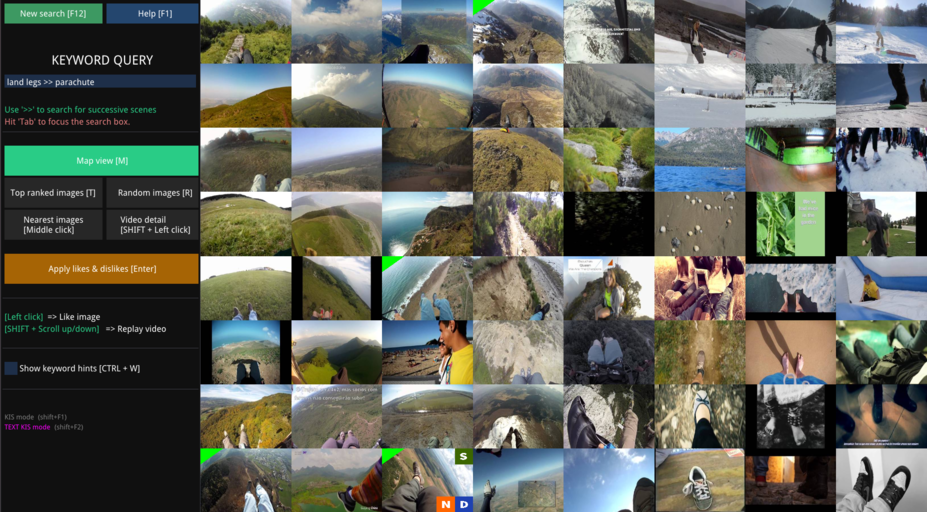
\includegraphics[width=0.99\linewidth]{img/som_hunter_small.png}
    \caption{A sample search in SOM Hunter. Source: \href{https://videobrowsershowdown.org/hall-of-fame/}{Video Broser Showdown, Hall of Fame}}
    \label{fig:som_hunter}
\end{figure}

\subsection{Vitrivr}

Vitrivr \citep{rossetto2016vitrivr} is a sophisticated framework for retrieving a video in the collection. Vitrivr is separated into three modules, Vitrivr-ng, Cineast, and Cottontail-DB.  Vitrivr-ng is the module responsible for creating queries that are later processed by the Cineast. Cottontail-DB supports fast retrieving methods of the features required by Cineast. The overview of the system is displayed in figure \ref{fig:vitrivr}. Vitrivr supports different query types, as query by a sketch, example image, semantic concept, keywords, audio, or motion. The feature extraction and the system behind retrieving the most similar results are parts of the second module -- Cineast (\cite{rossetto2016searching}). Cineast uses multiple approaches incorporating deep features, e.g., scene text recognition and speech-to-text recognition. Vitrivr-ng (the part responsible for creating the queries) is a web-based software. The modules structure provides a clean separation between the query formulation and feature extractions.

\begin{figure}
    \centering
    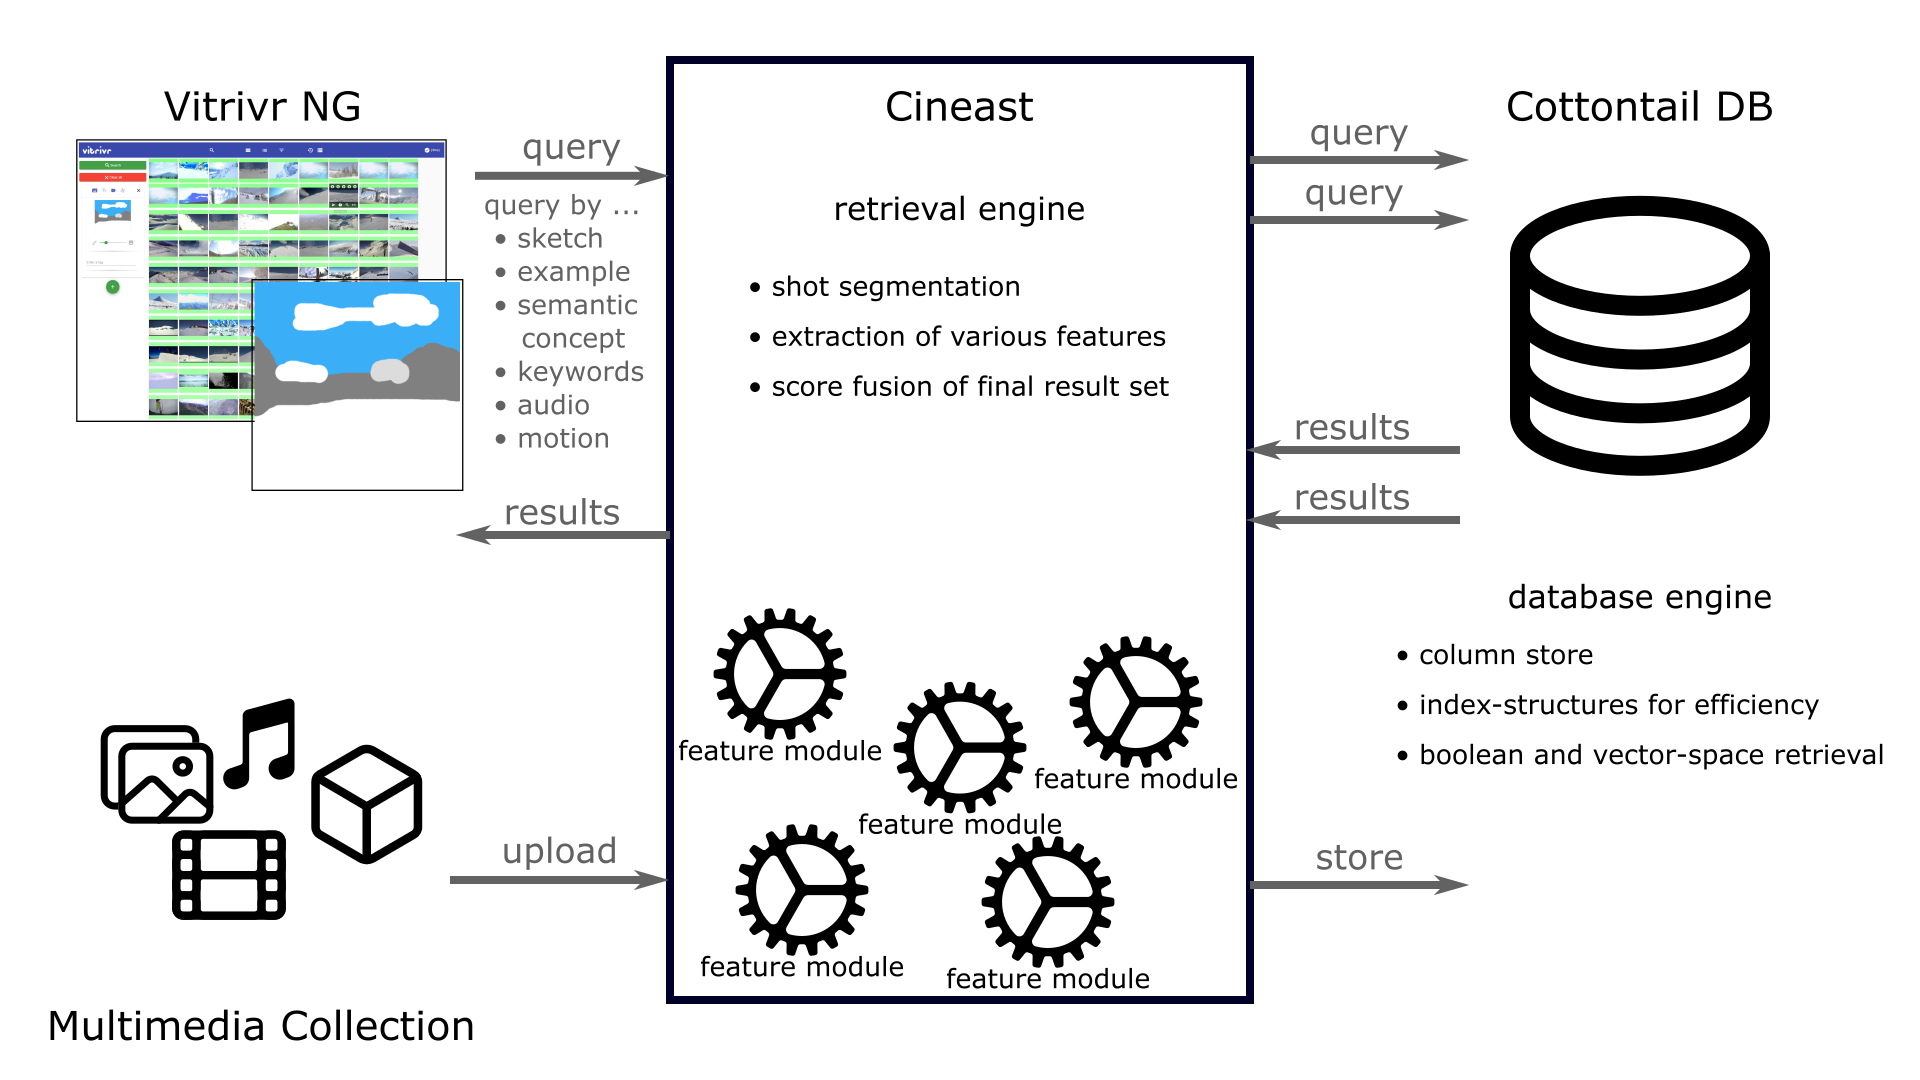
\includegraphics[width=\linewidth]{img/vitrivr.png}
    \caption{Overview of the separation in the Vitrivr framework. Source: \url{https://vitrivr.org/vitrivr.html}}
    \label{fig:vitrivr}
\end{figure}

\section{Deep Neural Networks}

In recent years we witnessed many records-breaking new machine learning models. Many of those were possible thanks to the advancement of Deep Neural Networks (DNN). Nowadays, these models replaced more traditional Machine Learning approaches in many tasks.

Deep Neural Network is a machine learning model, whose goal is to approximate a given function \(f\). The set of parameters is often referred to as \(\theta\). One of the everyday tasks performed by these networks is classification, where the goal of the network is to predict which category sample \(X\) belongs. Even though we will not perform a classification task in this thesis, we will use some of the available classification networks.

When we talk about neural networks, we usually refer to a feedforward network. These networks consist of layers which only pass information in one direction during the evaluation. We can imagine it as applying a function to the results from the previous layer. For example, let us create a small neural network. Denote first layer as \(f_1\) and second layer as \(f_2\). The output of the network will be \(f_2\left(f_1\left(\right)\right)\).

Stacking more and more layers on top of each other leads us to notation \emph{deep} neural networks. This notation has no fixed threshold on which networks "deserve" to be called deep. The word "deep" separates the eras between the neural networks from a few layers from neural networks consisting of tens or more layers.  

The first and last layer are commonly referenced as \emph{input} and \emph{output} layer, respectively. Layers between the input and output layers are usually denoted as \emph{hidden} layers. Deep neural networks can have four or hundreds of layers, and there multiple types of the operations that layer can perform. \emph{Network Architecture} captures the "build order" of the network. It is important to note that there exist many networks with different architectures solving the same task.

There are many reasons for the advancement of neural networks in the past years. One of the crucial stones was not only theoretical innovations used for the networks but increasing computability limits. Deep Neural Networks \emph{learn} to approximate function by \emph{training}. This training is usually the heaviest part of the computation. Even though it is enough to train once and use forever, it usually lays some limitations on the size of the networks or the functions used.

Since this topic is broad, we recommend more thorough reading, such as Neural Networks and Deep learning online book\footnote{http://neuralnetworksanddeeplearning.com/}.

\subsection{Convolution Neural Networks}

Convolution Neural Networks (CNN) are a class of Deep Neural Networks. Even though they emerged in the late 1980s \citep{lecun1989backpropagation}, it took another 20 years for further advancements in the research area. Convolution Neural Networks are mainly used in image-related tasks, such as image classification ("What is on the image?"), object detection ("Where are the objects in the image and what are they?") or even content generation ("Create a new image"). Their abilities were also tested in many, not image-related tasks, e.g., music genre recognition.

Convolutional Neural Networks are specialized kind of networks which work with grid-like topology. For 1D can be an example as time-series, or for 2D, most typically image pixels represent a grid. The name \emph{convolution} refers to using a mathematical linear function \emph{convolution} in at least the layers. A simplified overview of the structure is displayed in figure \ref{fig:convolution_neural_network}. We refer to \cite{Goodfellow-et-al-2016} for more understanding of \emph{convolutional layers}.

\begin{figure}
    \centering
    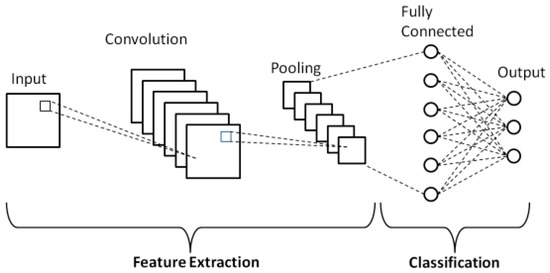
\includegraphics[width=0.98\textwidth]{img/convolution_neural_network.jpg}
    \caption{Schematic diagram of a convolutional neural network. Source: Phung, V.H.; Rhee, E.J. A High-Accuracy Model Average Ensemble of Convolutional Neural Networks for Classification of Cloud Image Patches on Small Datasets. Appl. Sci. 2019, 9, 4500.}
    \label{fig:convolution_neural_network}
\end{figure}

% \todo[inline]{pooling}
% \todo[inline]{convolution block}

\subsection{Transfer Learning}

Transfer Learning is a research problem in machine learning that focuses on storing knowledge gained while solving one problem and applying it to a different problem. We have seen many successful transfers of the network architecture and parameters learned to a new task. Transfer learning helps to reduce the cost of the training and often also to overcome an insufficient set of training examples for the new task.

We utilize some of the pre-trained Convolution Neural Networks. The ability of a convolutional neural network to transfer to a new task by elevating gained information from other datasets was explored as early as by \cite{donahuedeep}, and many others were able to use this information to gain better models.  Networks we use are mostly pre-trained on \emph{ImageNet}\footnote{http://www.image-net.org/}. ImageNet served as a benchmark for comparing the performance of the different networks. Since the ImageNet is the main classification task, we utilize the transfer learning in a way to obtain deep features. Layers to the end of the networks accumulate semantic information, i.e., they contain high-level features. Therefore, we work with the layers close to the end of the networks. These layers represent encoded information about the image in high dimensional vectors. Our task is to use these deep features obtained for solving our known-item search task.



\begin{figure}
    \centering
	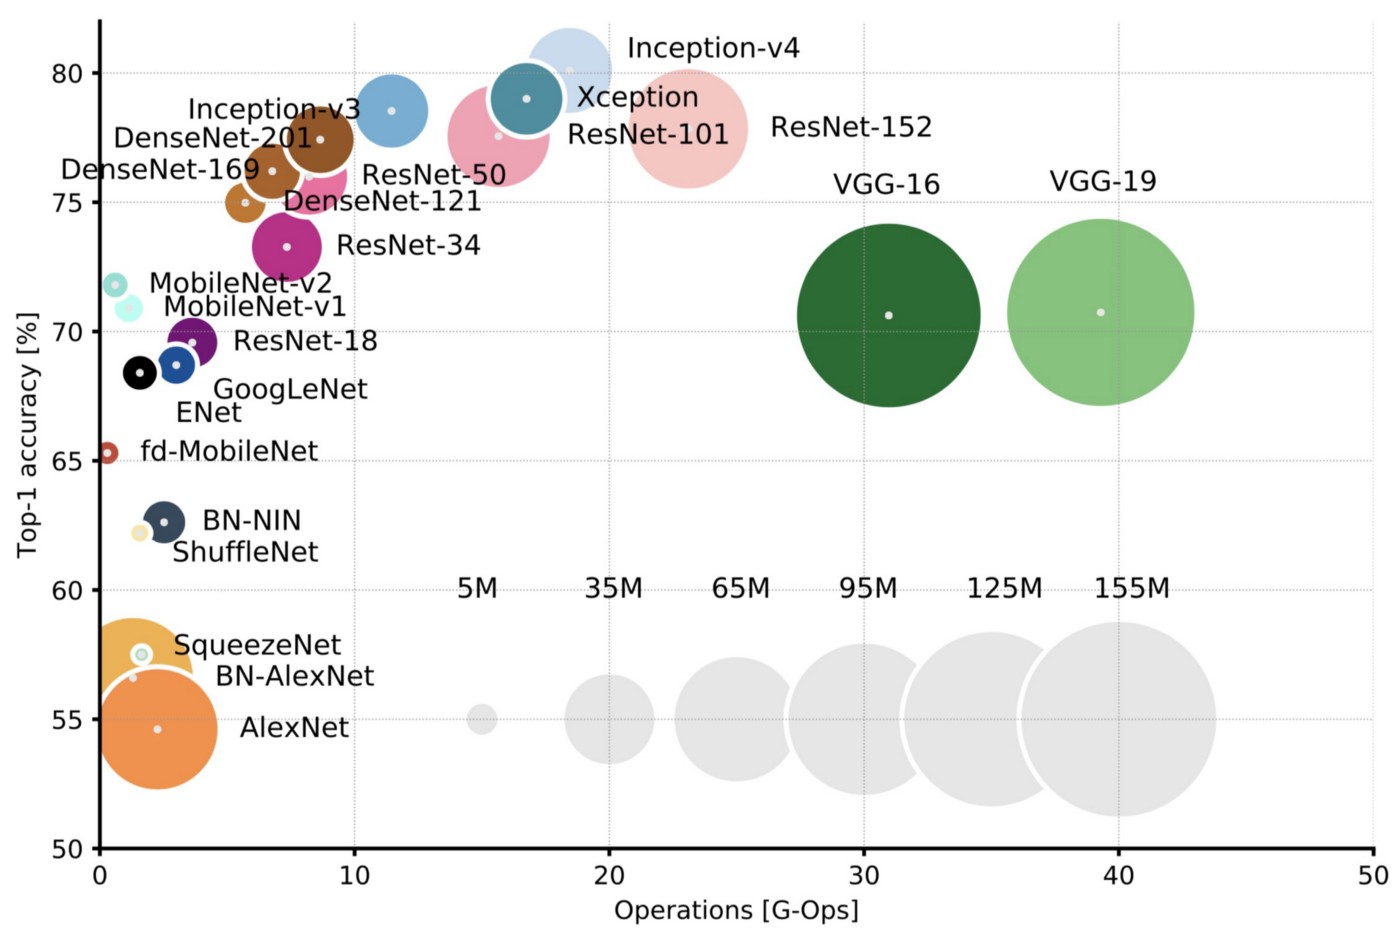
\includegraphics[width=0.8\linewidth]{img/network-comparison.jpeg}
	\caption{Top-1 one-crop accuracy versus amount of operations required for a single forward pass. The size of the blobs is proportional to the number of network parameters. Source: \cite{canziani2016analysis}}
	\label{fig:camera-setup}
\end{figure}

\subsection{Pretrained models}
\label{ss:pretrained_models}

\subsubsection{Keras}

Keras \citep{chollet2015keras} is a deep learning API written in Python, running on top of the machine learning platform TensorFlow \citep{tensorflow2015-whitepaper}. It was developed with a focus on experimentation in deep learning. We use it and its pre-trained models in this thesis. The models available in Keras Applications, which we use, were trained on ImageNet. Keras API allows us to separate the model from the last fully connected layer used for classification (since default ImageNet is a classification task). 

In this thesis, we use pre-trained models to implement new approaches. We do not aim to train new or further train existing models. We try to elevate the information from available models to solve the known-item search task. Here we describe two models, which we experimented most with. Firstly, ResNet was a state of the art model of 2015. Since then, it gained popularity in many tasks. The second network we focus on is MobileNet. MobileNet has an excellent performance to complexity ratio. Therefore, it is an ideal network for our purpose -- where the predictions need to be computed online and displayed to the user.

\subsubsection*{Resnet50V2}

ResNet (short for Residual Networks, \cite{resnet}) is a classic neural network used in many computer vision tasks. ResNet was the winner of the ImageNet challenge in 2015 and, therefore, state-of-art. ResNet architecture allowed to train deeper networks, which was not possible before because of vanishing gradients. ResNet's main idea is to allow "shortcuts" between the layers. This has two main reasons: it mitigates the problem of the vanishing gradients and allows to learn an identity function for higher layers in the network. ResNetV2 \citep{resnetv2} was released as an improvement of the ResNet. It included batch normalization and ReLU activation before 2D convolution. Also, a particularity of ResNetV2 included a residual branch.

ResNet is still well-known and popular among the machine-learning community. Several pre-trained models are available, and it has well-tested implementations. We use it in the thesis for some experiments, although we prefer MobileNet due to lower prediction time.

\subsubsection*{MobileNetV2}

In April 2017, a group of researchers from Google published a paper \citep{mobilenet} introducing a new architecture. This MobileNet was optimized for mobile devices. They optimized the model to deliver high accuracy while keeping the model and mathematical operations as fast as possible. Not a year later, MobileNetV2 was introduced by \cite{mobilenetv2}. It extended the predecessor using Inverted Residuals and Linear Bottlenecks (more in the paper). It improved the performance and therefore, we work only with MobilenetV2.


\subsubsection{Dlib}
Dlib \citep{king2009dlib} is a modern C++ toolkit containing machine learning algorithms and tools for creating complex software in C++ to solve real-world problems. Some of the modules are provided with Python API. We use the Dlib library for face detection and also face feature extraction. For both we use face\_recognition API \citep{geitgey2016machine}. \todo{fix ref \citep{king2017high} }


\section{Principal Component Analysis}

In this work, we perform Principal Component Analysis on a given set of features. The principal component analysis is one of the popular methods for dimensionality reduction. It uses Singular Value Decomposition (SVD) of the data to project it to a lower-dimensional space. Performing the PCA, we obtain features in lower-dimensional space, which contain most of the information from the original dataset. This has two advantages: the smaller feature vectors are faster to process, and it may even reduce the noise if present. Since the derivation of the formulas for PCA requires some basic knowledge of SVD and Linear Algebra, we refer to the \cite{alpaydin2020introduction} for a more detailed description.

\section{Dataset}
\label{s:dataset}

We use Vimeo Creative Commons Collections (V3C1)\footnote{\href{https://www-nlpir.nist.gov/projects/tv2019/data.html}{TRECVID 2019 Video Data}} dataset for experimenting and evaluations. The dataset is composed of 7475 Vimeo videos. We selected only the first 750 videos for proving concepts of our work. From these 750 videos, we used an extraction tool from VIRET \cite{lokovc2019framework}. After extraction, we obtained 111\ 764 images from 750 videos with resolution 320x180. I extend my gratitude to Tomáš Souček and Gregor Kovačík for providing extracted images.

The videos capture a wide range of sceneries on many different occasions. We can see many different landscapes, from seas to mountain views, from desert to snow. A large proportion of the videos contain people. Videos capture people doing different activities, i.e., from Hindi wedding to skateboarding in a park or a news broadcast.